% !TEX program = xelatex
\DocumentMetadata{lang=en} % required for transparent package
\documentclass[10pt,aspectratio=169]{beamer}
\newcommand{\subhead}[1]{\flushleft {\bf\large #1}\\}

% remove footcite numbers
\makeatletter
\def\@makefnmark{}
\makeatletter

\setbeamersize{text margin left=5mm,text margin right=5mm} 

\newcommand\focus[1]{%
	{\alert{\textbf{#1}}}
}

\usepackage{amsthm,amsmath,amssymb,braket,fontspec,unicode-math,fontenc,transparent}
\usepackage[absolute,overlay]{textpos}

\graphicspath{{./figures/}}
\usetheme[nofirafonts,numbering=none]{focus}
\setmainfont{Hero New}
\setsansfont{Hero New}
\setmathfont{Fira Math}

\usepackage[backend=bibtex,url=false,doi=false,style=authoryear]{biblatex}
\setbeamertemplate{bibliography item}{}
\bibliography{bib}
\AtBeginBibliography{\scriptsize}

\setbeamerfont{title}{size=\LARGE\scshape}
\setbeamerfont{author}{size=\Large}
\setbeamerfont{institute}{size=\large}
\setbeamerfont{date}{size=\large}
\setbeamerfont{frametitle}{size=\Large\scshape}
\setbeamerfont{sectiontitle}{size=\small\scshape}
\setbeamerfont{alerted text}{series=\bfseries}

\title{Pseudogapped Mott criticality: Stretching \\ Kondo Screening to Breaking Point}
\subtitle{How a Fermi liquid gives way to Mott insulator in 2D}

\author{Abhirup Mukherjee, Siddhartha Lal}

\institute
{
	Department of Physical Sciences,\\
	Indian Institute of Science Education and Research Kolkata
}
\date{\today}
\titlegraphic{
	\vspace{80pt}
	
\includegraphics[width=0.08\textwidth]{epqm_logo_mod.jpeg}\hspace*{20pt}
\includegraphics[width=0.08\textwidth]{dps_logo.jpeg}\hspace*{350pt}
}

\begin{document}

\begin{frame}
    % Print the title page as the first slide
    \titlepage
\end{frame}

\begin{frame}{Some Questions}
\footcite{keimer2015quantum,ProustTaillefer2019,loeserKapitulnik1996,Norman1998,Hashimoto2014,KyungKotliar2006,MacridinAzevedo2006,WuFerrero2018,anirbanmott2,HilleAndergassen2020}
The anomalous \alert{pseudogap} (PG) phase exhibits nodal-antinodal dichotomy.\\[5pt]

No general consensus yet regarding
\begin{itemize}
	\item nature of \(T=0\) ground states of the cuprates
	\item \alert{relation} of PG to Mott insulating and superconducting phases proximate to it
	\item how pseudogap \alert{evolves} from weak- to strong-coupling
	\item nature of correlations and entanglement within the transition
to the model
\end{itemize}

\begin{center}
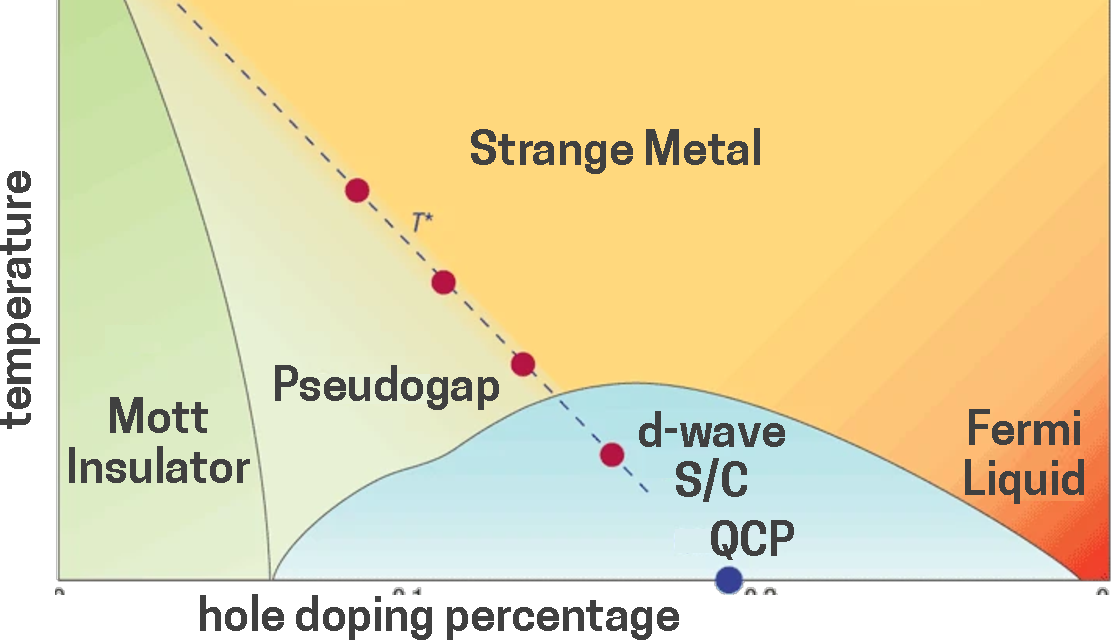
\includegraphics[height=0.2\textwidth]{cuprates.pdf}
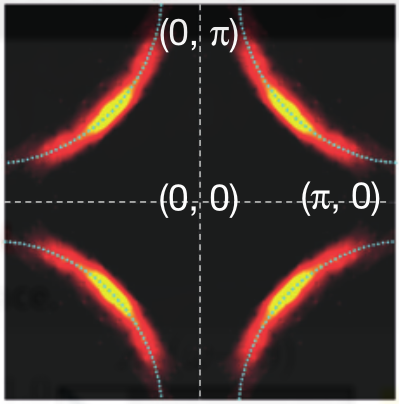
\includegraphics[height=0.2\textwidth]{fermiArc1.png}
\end{center}

\end{frame}

\begin{frame}{New Auxiliary Model Approach To Interacting Fermions}
	\footcite{stoyanova,Maier2005,Sakai2023}
	\begin{minipage}{0.4\textwidth}
		1. Solve an appropriate \alert{impurity model}, \(H_\text{imp}\)
	\begin{itemize}
		\item Lattice symmetry
		\item Impurity phase transition
	\end{itemize}
	\end{minipage}
	\hfill
	\begin{minipage}{0.48\textwidth}
		2. \alert{Construct lattice} model by applying manybody translation operators:
	\[ H_\text{latt} = \sum_{\bf r} T^\dagger({\bf r}) H_\text{imp}({\bf r_0})T({\bf r})\]
	\end{minipage}

	\vfill
	3. Relate computables across the models, using manybody Bloch's theorem\\[5pt]
	\begin{minipage}{0.55\textwidth}
	\alert{Greens functions}: \\
	\[\tilde G({\bf K}\sigma; \omega) = G^>(\mathcal{T}^\dagger_{{\bf K}\sigma}, \omega - \varepsilon_{{\bf K}}) + G^<(\mathcal{T}^\dagger_{{\bf K}\sigma}, \omega + \varepsilon_{{\bf K}})\]
	Equal-time \alert{correlation} functions:
	\[C_{\mathcal{O}}({\bf k}_1,{\bf k}_2) = \sum_{{\Delta}}\braket{{\bf r}_c + {\Delta} | \mathcal{\tilde O}({\bf k}_2) | {\bf r}_c}\braket{{\bf r}_c | \mathcal{\tilde O}^\dagger({\bf k}_1) | {\bf r}_c}\]
	\end{minipage}
	\hfill
	\begin{minipage}{0.43\textwidth}
		where \\[5pt]
		\(G^>(\mathcal{O}^\dagger, t) = -i\braket{\mathcal{O}(t)\mathcal{O}^\dagger}\)\\[5pt]
		\(\mathcal{T}_{{\bf K}\sigma} = c_{{\bf K}\sigma}\left(\sum_{\sigma^\prime}c^\dagger_{d\sigma} + \text{h.c.}\right) + c_{{\bf K}\sigma}\left(S_d^+ + \text{h.c.}\right)\)\\[5pt]
		\(\mathcal{\tilde O}({\bf r}) = \mathcal{O}({\bf r})\mathcal{O}^\dagger(d)\)
	\end{minipage}
	
	
	
\end{frame}

\begin{frame}{The Core Ingredient: A Lattice-Embedded Impurity Model}
	\footcite{Yang2002}
\begin{minipage}{0.75\textwidth}
	\vspace{-10pt}
	\[\mathcal{H}_\text{imp} = H_\text{2D-TB-KE} + V\sum_{Z,\sigma} \left(c^\dagger_{d\sigma}c_{Z\sigma} + \text{h.c.}\right) + J\sum_{Z} {\bf S}_d\cdot {\bf S}_Z -\frac{W}{2}\sum_{Z} \left(n_{Z\uparrow} - n_{Z\downarrow}\right)^2\]
	\vspace{-10pt}
	\begin{itemize}
		\item \(J_{{\bf k}, {\bf k}^\prime}\) has \alert{\(C_4-\)symmetry} instead of \(s-\)wave symmetry
	\end{itemize}
	\(J_{{\bf k}, {\bf k}^\prime} = \frac{J}{2}\left[\cos\left({\bf k}_x - {\bf k}^\prime_x\right) + \cos\left({\bf k}_y - {\bf k}^\prime_y\right)\right]\)
\end{minipage}
\begin{minipage}{0.2\textwidth}
	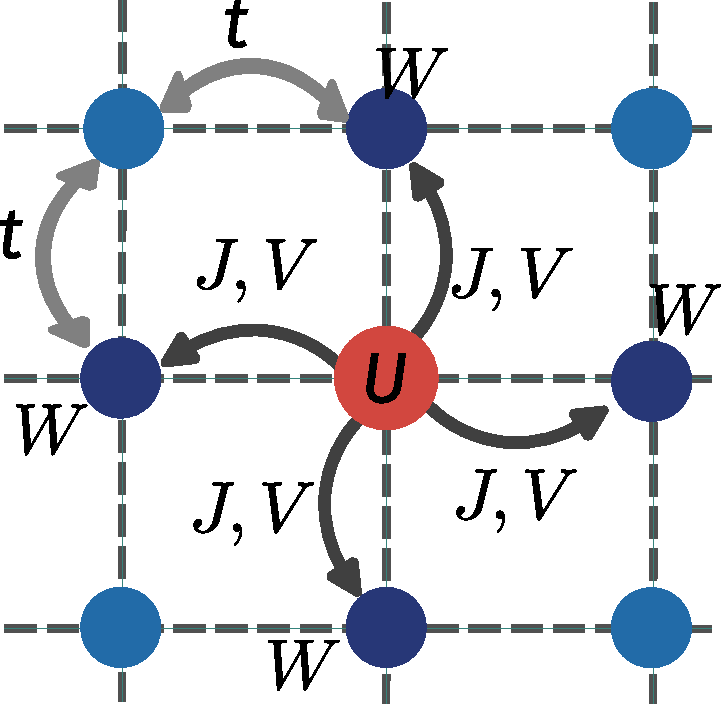
\includegraphics[width=\textwidth]{pWaveEsiam.pdf}
\end{minipage}

\vspace{10pt}
\uncover<2-3>{
\alert{Map to Hubbard-Heisenberg Model}

\begin{minipage}{0.45\textwidth}
% \vspace{5pt}
\begin{equation*}\begin{aligned}
	&\mathcal{H}_\text{latt} = \sum_{\bf r} T^\dagger({\bf r}) H_\text{imp}({\bf r_0})T({\bf r}) \\[-5pt]
	&= -\frac{\tilde t}{\sqrt{\mathcal{Z}}} \sum_{\left<{\bf r}_i, {\bf r}_j\right>;\sigma}\left(c^\dagger_{{\bf r}_i,\sigma}c_{{\bf r}_j,\sigma} + \text{h.c.}\right) - \tilde \mu \sum_{{\bf r}}\hat n_{{\bf r},\sigma} \\[-5pt]
	&+ \frac{\tilde J}{\mathcal{Z}}\sum_{\left< {\bf r}_i, {\bf r}_j\right>}{\bf S}_{{\bf r}_i}\cdot{\bf S}_{{\bf r}_j} - \frac{1}{2}\tilde U\sum_{\bf r}\left(\hat n_{{\bf r} , \uparrow} - \hat n_{{\bf r} , \downarrow}\right)^2
\end{aligned}\end{equation*}
\end{minipage}
\hfill
\begin{minipage}{0.18\textwidth}
\[\tilde t = t+2V\]
\[\tilde U = U + W\]
\[\tilde \mu = 2\mu + \eta,~ ~ \tilde J = 2J\]
\end{minipage}
\hfill
\uncover<3>{
\begin{minipage}{0.3\textwidth}
	\begin{itemize}
		\item We work in large \(U\) limit
		\item SW transformation \(\to\) \alert{\(J-W\) model}
	\end{itemize}
	
\end{minipage}
}
}
\end{frame}

\begin{frame}{Pseudogapping Transition from Kondo Breakdown}
\begin{minipage}{0.48\textwidth}
Unitary RG analysis - integrate out high-energy states in the conduction bath:
\[\Delta J^{(j)}_{{\bf k}_1, {\bf k}_2} = -\sum_{{\bf q} \in \text{PS}} \frac{J^{(j)}_{{\bf k}_2,{\bf q}} J^{(j)}_{{\bf q},{\bf k}_1} + 4J^{(j)}_{{\bf q}, {\bf \bar q}} W_{{\bf \bar q}, {\bf k}_2, {\bf k}_1, {\bf q}}}{\omega - \frac{1}{2}|\varepsilon_j| + J^{(j)}_{{\bf q}}/4 + W_{{\bf q}}/2}\]
\end{minipage}
\begin{minipage}{0.48\textwidth}
	\begin{itemize}
	\uncover<2->{\item momentum-\alert{anistropic} screened phase between SC and LM phases.}
	\uncover<3->{\item Impurity-bath spin correlations show \(k-\)differentiation}
	\uncover<4->{\item Lattice model DOS shows \alert{P-gap}}
	\end{itemize}
\end{minipage}
	
\begin{center}
	\uncover<2->{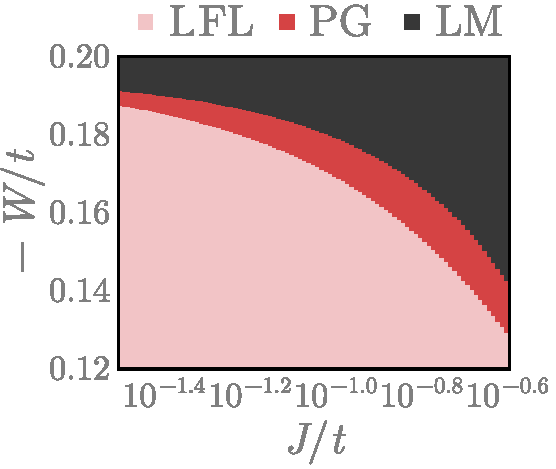
\includegraphics[width=0.32\linewidth]{phaseDiagram.pdf}}
	\uncover<3->{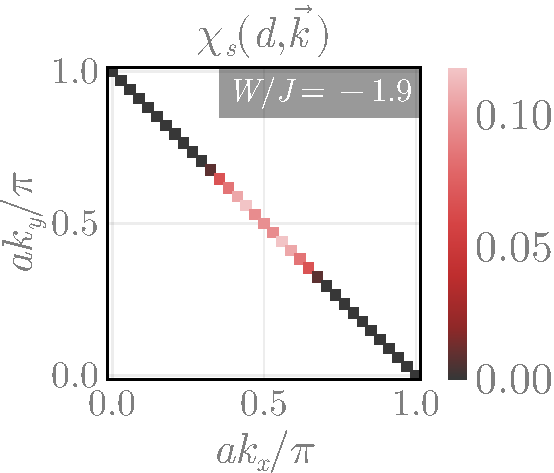
\includegraphics[width=0.32\linewidth]{SF-3.pdf}}
	\uncover<4->{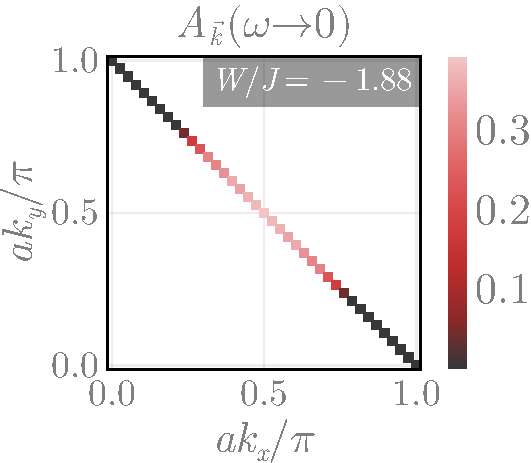
\includegraphics[width=0.32\linewidth]{kspaceDOS-3.pdf}}
\end{center}
\end{frame}

\begin{frame}{Unravelling of Kondo screening}
	The Kondo breakdown process can be visualised in terms of \alert{zeros} of $J_{{\bf k}_N, {\bf k}}$.
\begin{itemize}[<+->]
	\item $J_{{\bf k}_N, {\bf k}}$ for ${\bf k}$ close to the \alert{adjacent nodes} turn RG irrelevant first, and a patch of zeros subsequently appears in $J_{{\bf k}_N, {\bf k}}$ around this point. 
	\item Tuning $W/J$ further extends the patch of zeros in $J_{{\bf k}_1, {\bf k}_2}$ for all ${\bf k}_{1}$ lying between a given node and the nearest antinodes. 
	\item At $W=W_{\text{PG}}$, the \alert{antinode} joins this connected region of zeros in $J_{{\bf k}_1, {\bf k}_2}$, marking the onset of the PG.
\end{itemize}

\begin{center}
    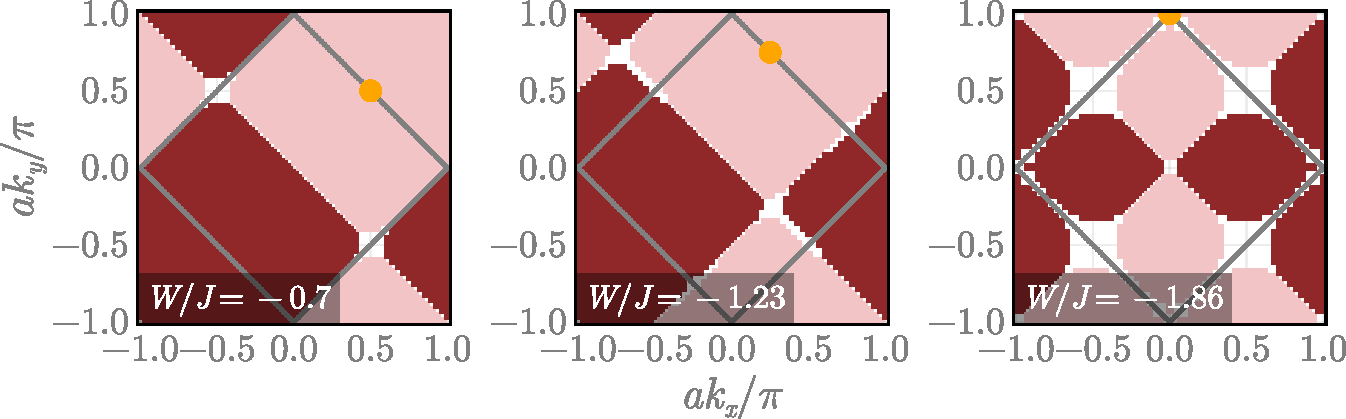
\includegraphics[width=0.8\linewidth]{zerosFlow.pdf}
\end{center}

\end{frame}

\begin{frame}{Dynamical Spectral Weight Transfer}
\begin{itemize}
	\item strong fluctuations observed in \alert{charge correlations} between the gapless nodal and gapped antinodal regions in PG regime
	\item PG formation results from the \alert{transfer of spectral weight} from low to high energies
	\item PG coincides with the appearance of poles of the lattice model self-energy $\Sigma ({\bf k},\omega=0)$ near the antinodes
\end{itemize}

\begin{center}
	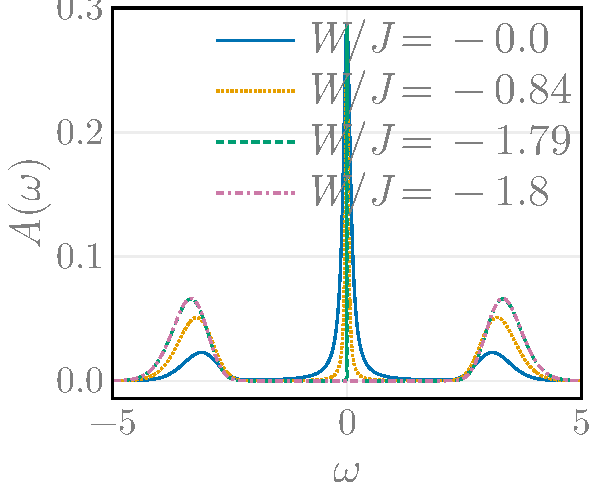
\includegraphics[width=0.32\linewidth]{impSpecFunc_49-1000.pdf}
    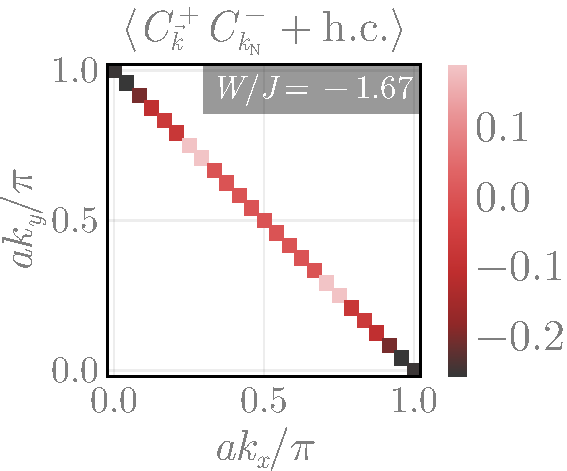
\includegraphics[width=0.32\linewidth]{cfnode-2.pdf}
    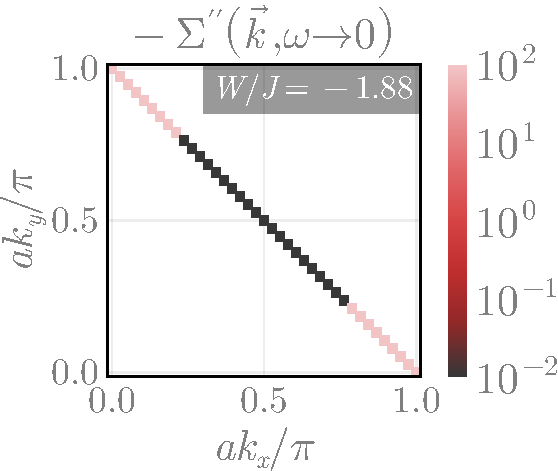
\includegraphics[width=0.32\linewidth]{selfEnergyKspace-3.pdf}
\end{center}
\end{frame}


\begin{frame}{Non-Fermi liquid nature of the pseudogap}
	\begin{itemize}
		\item In PG phase, Kondo processes between adjacent \(k-\)space quadrants are removed at low-energies
		\item Effective \alert{two-channel Kondo} description - each pair of opposite quadrants forms a channel
		\item \alert{Non-Fermi liquid} physics - vanishing quasiparticle residue, and \(\Sigma\) poles near \(\omega=0\)
	\end{itemize}
	
\vspace{-5pt}
\begin{center}
	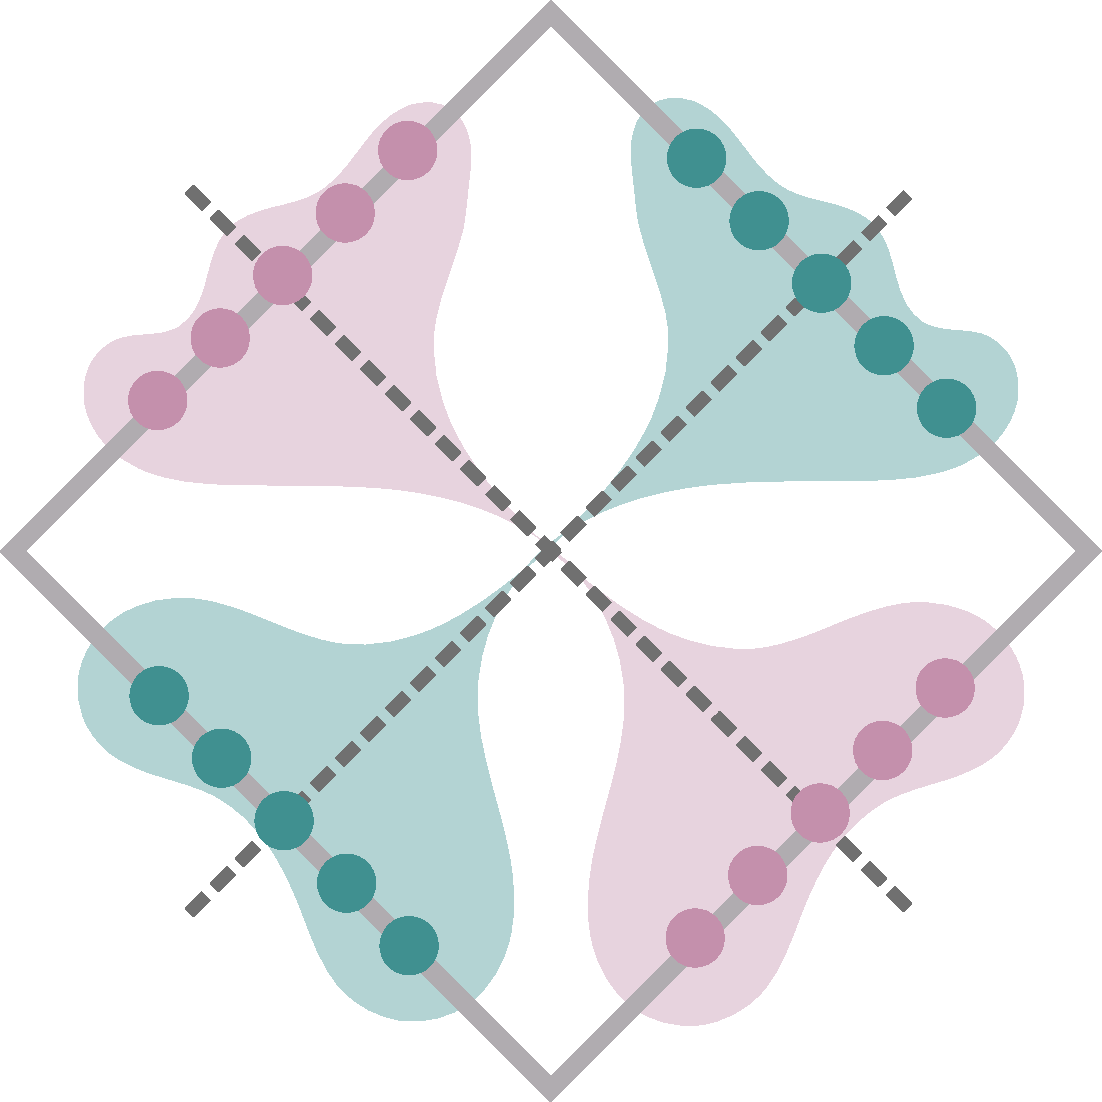
\includegraphics[width=0.32\linewidth]{twoChannel.pdf}
    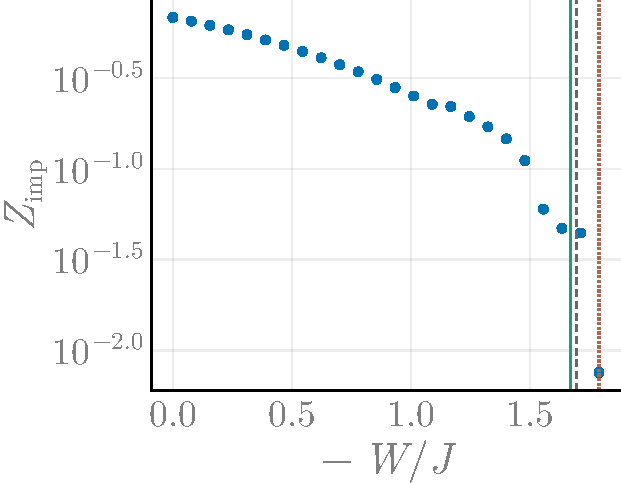
\includegraphics[width=0.32\linewidth]{localQPResidue.pdf}
    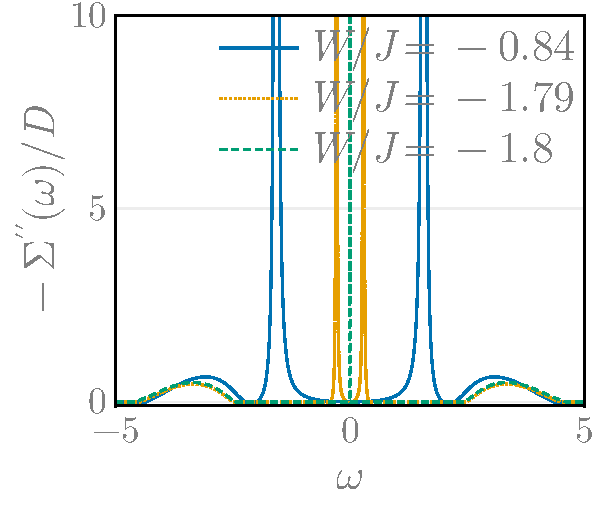
\includegraphics[width=0.32\linewidth]{sigmaImag_49-1000.pdf}
\end{center}
\end{frame}

\begin{frame}{Singular Nodal Metal}
	\begin{minipage}{0.3\textwidth}
	\uncover<1->{
		\only<1>{
		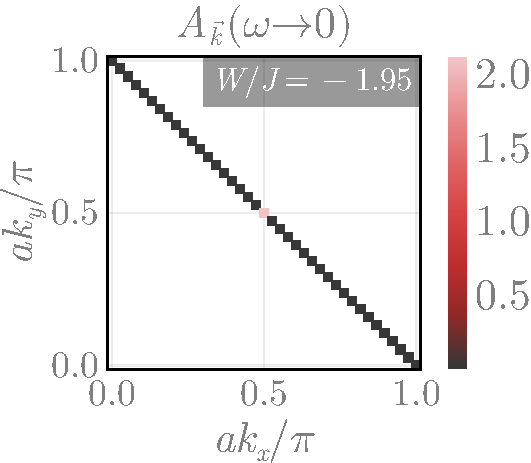
\includegraphics[width=\linewidth]{kspaceDOS-4.pdf}
		}
		\only<2->{
		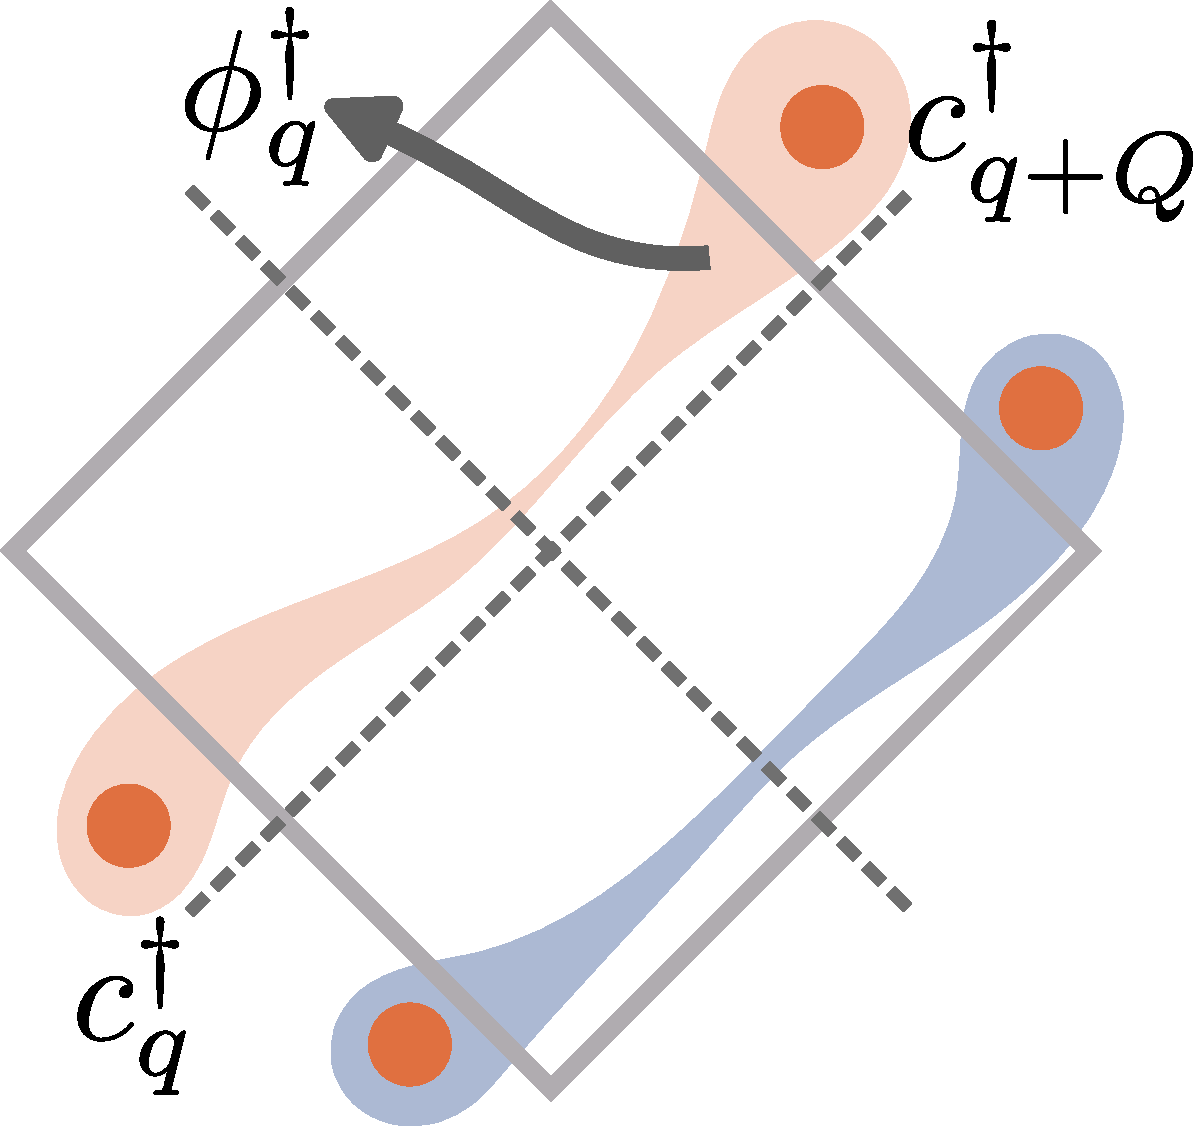
\includegraphics[width=\linewidth]{phiMode.pdf}
		}
	}
	\end{minipage}
	\hfill
	\only<1->{
	\begin{minipage}{0.65\textwidth}
		Close to the transition, Kondo cloud consists of concentrated \alert{nodal regions}\\[5pt]
		Low-energy excitations
		\begin{itemize}
			\item Integrate out impurity spin-flips (\(~ J^2/W\))
			\item SW transformation \(\to\) effective Hamiltonian
		\end{itemize}

		\vspace{5pt}
		\uncover<2->{
			Emergent modes: \( \phi_{{\bf q}, \sigma} = \frac{1}{\sqrt 2}\left(c_{{\bf N}_1 + {\bf q},\sigma} - c_{{\bf N}_1 + {\bf Q}_1 - {\bf q}, \sigma}\right),~r = \phi^\dagger \phi\)
		}
	\end{minipage}
	}
	\uncover<3->{
		\[ \Delta \tilde H = \underbrace{\sum_{{\bf q}, \sigma}\frac{|\varepsilon_{{\bf N}_1 + {\bf q}}|\varepsilon_{{\bf N}_1 + {\bf q}}}{-W} r_{{\bf q},\sigma}}_\text{dispersion} + \sum_{{\bf q}_1,{\bf q}_2, \sigma}\frac{{J^*}^2}{-4W}\left[\underbrace{r_{{\bf q}_1 \sigma} \left(1 - r_{{\bf q}_2 \bar\sigma}\right)}_\text{density interaction} - (1 - \delta_{{\bf q}_1,{\bf q}_2})\underbrace{\phi^\dagger_{{\bf q}_1,\bar\sigma}\phi^\dagger_{{\bf q}_1,\sigma}\phi_{{\bf q}_2, \sigma}\phi_{{\bf q}_2, \bar\sigma}}_\text{fwd/tang. pair transfer}\right] \]
	}
	
\end{frame}

\begin{frame}{Singular Nodal Metal: \(q_1 = q_2\)}
	We focus on the simplified case of zero momentum transfer \(q_1=q_2\):
	\[ \Delta \tilde H = \sum_{{\bf q},\sigma}\epsilon_{{\bf q}}{r}_{{\bf q},\sigma} + u\sum_{{\bf q}, \sigma}r_{{\bf q} \sigma} r_{{\bf q} \bar\sigma},\quad\phi_{{\bf q}, \sigma} = \frac{1}{\sqrt 2}\left(c_{{\bf N}_1 + {\bf q},\sigma} - c_{{\bf N}_1 + {\bf Q}_1 - {\bf q}, \sigma}\right),~r = \phi^\dagger \phi \]
	\[\epsilon_{\bf q} = \frac{|\varepsilon_{{\bf N}_1 + {\bf q}}|\varepsilon_{{\bf N}_1 + {\bf q}}}{-W} + \frac{{J^*}^2}{-4W},~u = \frac{{J^*}^2}{4W}\]
	\begin{itemize}
		\item Nodal metal is described by a \alert{Hatsugai-Kohmoto model}.
		\item Non-Fermi liquid excitations.
	\end{itemize}
	\[\Sigma \sim \frac{u^2}{\omega}, Z \sim \omega^2\]
	
\end{frame}

\begin{frame}{Non-local nature of the pseudogap}
\begin{itemize}
	\item real-space correlations and entanglement undergo a crossover within the pseudogap from short-ranged to \alert{long-ranged} behaviour\\[5pt]
	\item This is further evidence of the \alert{breakdown of local Kondo screening}, and resulting Landau quasiparticle excitations\\[5pt]
	\item the Mott transition observed by us for the Hubbard-Heisenberg model on the square lattice lies well beyond the paradigm of \alert{local quantum criticality}
\end{itemize}

\begin{center}
    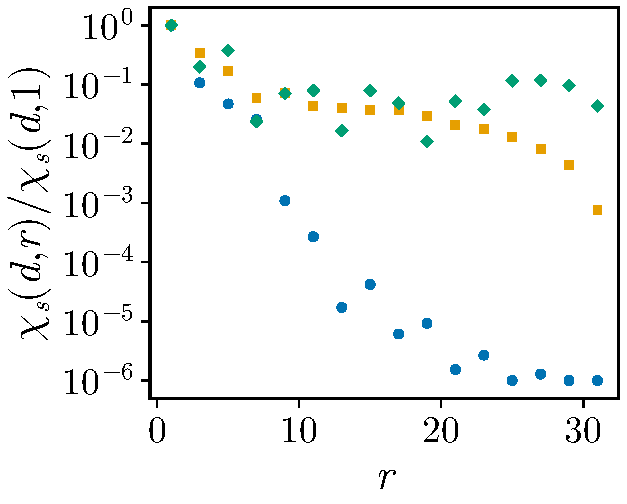
\includegraphics[width=0.35\linewidth]{SF-di_69-2000.pdf}
    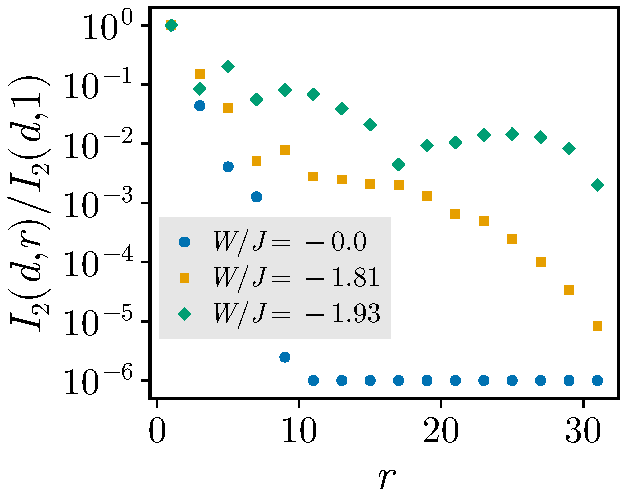
\includegraphics[width=0.35\linewidth]{I2-di_69-2000.pdf}
\end{center}
\end{frame}

\begin{frame}{Conclusions}
	\begin{itemize}
		\item On a 2D square lattice, a Fermi liquid must morph into a \alert{non-Fermi liquid pseudogap phase} in order to give rise to a Mott insulator
		\item $k-$space differentiated \alert{Kondo breakdown} lies at the heart of this physics
		\item the pseudogap features increasingly \alert{non-local correlations} as the system is driven towards the transition
	\end{itemize}

	\vfill
	{\large \alert{Future Directions}}
	\begin{itemize}
		\item Heavy fermions?
		\item Doping the pseudogap phase?
		\item Other impurity model geometries - spin liquids?
	\end{itemize}

\end{frame}


\end{document}
